\documentclass[dvipsnames]{beamer}
\usepackage[utf8]{inputenc}

\usepackage{./beamerthemeCourse}
\usepackage{listings}
\lstset{language = Tex}

\usepackage[absolute,overlay]{textpos}
\usepackage[normalem]{ulem}
\usepackage{numprint}       % Histoire que les chiffres soient bien

\usepackage{amsmath}        % La base pour les maths
\usepackage{amsthm}
\usepackage{mathrsfs}       % Quelques symboles supplémentaires
\usepackage{amssymb}        % encore des symboles.
\usepackage{amsfonts}       % Des fontes, eg pour \mathbb.
\usepackage{rotating}

% ---- IMPOSTAZIONI PRESENTAZIONE ----
\title{Tabelle nel mondo \LaTeX}
\subtitle{Tabelle semplici, con bordi, su più pagine }
\author{F. Fasolato, G. Zecchin, Guido Sportivo, A. Bari}
\date{AA 2018-2019}

% ---- IMPOSTAZIONI PACCHETTI ----
\definecolor{forestgreen}{rgb}{0.13, 0.55, 0.13}

\lstset{
    language=[LaTeX]Tex,%C++,
    keywordstyle=\color{blue}, %\bfseries,
    basicstyle=\small\ttfamily,
    commentstyle=\color{forestgreen}\ttfamily,
    stringstyle=\rmfamily,
    numbers=left,%
    numberstyle=\scriptsize, %\tiny
    stepnumber=1,
    numbersep=8pt,
    showstringspaces=false,
    breaklines=true,
    frameround=ftff,
    frame=single
}

\usepackage{beamerthemeCourse}
\usepackage[T1]{fontenc}
\usepackage[utf8]{inputenc}
\usepackage[absolute,overlay]{textpos}
\usepackage{listingsutf8}
\usepackage{listings}

% ---- IMPOSTAZIONI PACCHETTI ----
\definecolor{forestgreen}{rgb}{0.13, 0.55, 0.13}

\lstset{
    language=[LaTeX]Tex,%C++,
    keywordstyle=\color{blue}, %\bfseries,
    basicstyle=\small\ttfamily,
    commentstyle=\color{forestgreen}\ttfamily,
    stringstyle=\rmfamily,
    numbers=left,%
    numberstyle=\scriptsize, %\tiny
    stepnumber=1,
    numbersep=8pt,
    showstringspaces=false,
    breaklines=true,
    frameround=ftff,
    frame=single,
    inputencoding=utf8/latin1
}   

\title{Package, theme e template}
\subtitle{Utilizzo di temi e modelli preimpostati per decorare il documento}
\author{F.Fasolato, G.Zecchin, G.Santi, A.Bari}
\date{AA 2018-2019}





\begin{document}

	\maketitle
	\begin{frame}{Outline}
        \tableofcontents
    \end{frame}
	\section{Package}
\begin{frame}{Package}

\begin{itemize}
\item I \emph{package} possono essere visti come delle raccolte di funzionalità a cui possiamo accedere durante la scrittura di un documento

\vfill

\item Per usare un package il comando è 
\texttt{\textbackslash{}usepackage\{nome\_package\}}

\vfill

\item I package permettono di inserire immagini, cambiare il colore del testo,
inserire URL\dots{}

\end{itemize}

\end{frame}
	\begin{frame}[fragile]{Esempio (1)}

\begin{esempio}{Senza l'utilizzo di package}
	\begin{code}
	    \inputminted[linenos] {latex}{res/examples/withoututf8.tex}
	\end{code}

\pause
	
	\begin{figure}
        \centering
        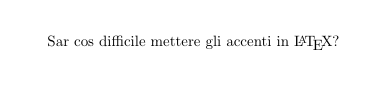
\includegraphics[scale=0.9]{res/images/no_utf8}
    \end{figure}
    \vspace{1mm}
\end{esempio}

\end{frame}

	\begin{frame}[fragile]{Esempio (2)}

\begin{esempio}{Con l'utilizzo di package}
    \begin{code}
        	\inputminted[linenos] {latex}{res/examples/withutf8.tex}
    \end{code}
    
	\begin{figure}
        \centering
        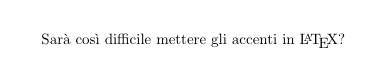
\includegraphics[scale=0.9]{res/images/w_utf8}
    \end{figure}
    \vspace{1mm}
\end{esempio}

\end{frame}

	\begin{frame}{Theme}

\section{Theme}
\begin{figure}
	\centering
	
\includegraphics[scale=0.20]{res/images/temi}
\end{figure}

\begin{itemize}
	\item Si parla di temi invece nel caso di presentazioni \texttt{beamer}
	\item Anche in questo caso è possibile definirne uno proprio ma non lo
	faremo
	\item È possibile applicare un tema usando il comando
	\texttt{\textbackslash{}usetheme\{nome\_pacchetto\}}
	\item Certi temi permettono di scegliere la gamma di colori sfruttando il
	comando \texttt{\textbackslash{}usecolortheme\{nome\_colore\}}
\end{itemize}

\end{frame}
	\section{Newcommand}
\begin{frame}{Newcommand 1}



Nei file di grandi dimensioni, spesso \`e necessario ripetere pi\`u volte una parola, una frase o un pezzo di codice. Per evitare Copy \& Paste inutili \LaTeX{} ha introdotto l'istruzione \mintinline{latex}{\newcommand{nome_comando}{testo visualizzato}}.
\begin{esempio}{New command 1}
\codedInput{res/examples/command.tex}

\end{esempio}

Il testo visualizzato sar\`a: $\R$.

\end{frame}

\begin{frame}{Newcommand 2}

\mintinline{latex}{\newcommand} pu\`o accettare anche dei parametri. Grazie all'utilizzo delle parentesi quadre si pu\`o definire:


\begin{esempio}{New command 2}
\codedInput{res/examples/command2.tex}
\end{esempio}
Questo comando pu\`o essere utilizzato per vari simboli:
\begin{itemize}
    \item $\bb{C}$
    \item $\bb{R}$
    \item $\bb{Z}$
    \item ...
\end{itemize}
\end{frame}

\begin{frame}{Newcommand 3}

\mintinline{latex}{\newcommand} pu\`o accettare anche delle opzioni:

\begin{esempio}{New command 3}
\codedInput{res/examples/command3.tex}
\end{esempio}
dove:
\begin{itemize}
    \item[\textbf{[3]}] Rappresenta il numero di parametri
    \item[\textbf{[2]}] \`E il valore di default del primo parametro
    \item[\#N] Rappresenta il parametro N
\end{itemize}
Quindi il comando \mintinline{latex}{\plusbinomial{x}{y}} viene visualizzato come:
\begin{center}
    $\plusbinomial{x}{y}$
\end{center}


\end{frame}
\section{Renew Command}
\begin{frame}{Renew Command}

Cos\`i come \`e possibile definire nuovi comandi \`e anche possibile ridefinire i comandi esistenti, siano essi definiti dall'utente o siano quelli di default.

\begin{esempio}{Renew Command}
\codedInput{res/examples/renew.tex}
\end{esempio}
Quindi il comando \mintinline{latex}{\LaTeX} ora viene visualizzato come:
\LaTeX.

\end{frame}
	\section{Esercizi}
\begin{frame}{Esercizi}

\begin{esercizio}{Esercizio 1}
\mInput{res/examples/excercise1.tex}
\end{esercizio}
\begin{esercizio}{Esercizio 2}
Definire il comando \mintinline{latex}{\add} che prende due parametri e produce il seguente output:\\
\centering
\add{1}{2}
\end{esercizio}
\end{frame}

\begin{frame}{Esercizi 2}
\begin{esercizio}{Esercizio 3}
Definire il comando \mintinline{latex}{\price} che ha il seguente comportamento:
\begin{itemize}
\item \mintinline{latex}{\price{100}} produce \price{100}
\item \mintinline{latex}{\price[20]{100}} produce \price[20]{100}

\end{itemize}
\end{esercizio}


\end{frame}
	\section{Environment}
\begin{frame}{New Environment}

Analogamente a quanto abbiamo appena visto per i comandi \`e possibile definire e ridefinire gli environment:

\begin{esempio}{New Environment}
\codedInput{res/examples/environment.tex}
\end{esempio}

\end{frame}

\begin{frame}{New Environment 2}

\begin{esempio}{Code block}
\codedInput{res/examples/codeblock.tex}
\end{esempio}
Viene visualizzato come:
\begin{ourboxed}{Title of the Box}
This is the text formatted by the boxed environment
\end{ourboxed}

\end{frame}
	\section{Template}
\begin{frame}{Template}

\begin{itemize}
\item I \emph{template} invece possiamo pensarli come delle raccolte di comandi
che definiscono l'aspetto e i possibili comandi per un certo documento
\item Possono definire anche i pacchetti utilizzati
\item Non definiremo mai un template ma ce ne sono moltissimi disponibili online
    \subsection{Esempio di template per la tesi}
\item \textbf{Vediamo un esempio di template per la tesi!}
\end{itemize}

\begin{figure}
	\centering
	
\includegraphics[scale=0.20]{res/images/template}
\end{figure}

\end{frame}

	

\end{document}
